% LTeX: language=de-DE
\chapter{Mechanik}
	Wie in \cref{sec:constructive limitations} besprochen, beschränkt sich die Auswahl möglicher Antriebselemente praktischerweise auf BLDC-Motoren, die wiederum auf dem Markt als \textit{Inrunner} und \textit{Outrunner} erhältlich sind.
	In ersteren sind die Statorwicklungen an der Außenseite angeordnet, zweitere ordnen sie an der Innenseite an.
	\begin{figure}[h]
		\centering
		\includesvg[width=.8\textwidth]{Assets/Inrunner_Outrunner}
		\caption[Gegenüberstellung von Inrunner und Outrunner]{Schematische Gegenüberstellung von BLDC-Motoren als Inrunner (links) bzw. Outrunner (rechts) ausgeführt~\cite{inrunner.outrunner.2022}.}%
		\label{fig:inrunner outrunner}
	\end{figure}
	Das Funktionsprinzip bleibt so zwar unverändert, durch den vergrößerten Radius des Angriffspunktes der magnetischen Kopplung kann bei gleicher Baugröße und gleichem Phasenstrom allerdings ein höheres Drehmoment erzeugt werden.
	Sind größere Drehzahlen gefordert, so ist die Bauweise des Inrunners durch den reduzierten Durchmesser des Rotors vorteilhaft.
	Da hohe Drehzahlen gegenüber einem zu erzeugenden Drehmoment für das zu konstruierende Antriebssystem von untergeordneter Priorität sind und sich oberhalb eines Schwellwertes sogar kontraproduktiv auswirken können, fällt hier die Wahl auf das Outrunnerprinzip.\par\medskip
	%
	Auch während Lenkmanövern muss eine Übertragung des Drehmomentes auf die Rollen der Trucks sichergestellt sein.
	Praktikabel und mit einfachen Mitteln denkbar sind hier eine koaxiale Positionierung des Motors zur angetrieben Rolle.
	Der Motor kann hier unter eines Offsets weiter im Zentrum des Hangers platziert werden, setzt in dem Fall jedoch eine Hohlwelle zwingend voraus.\par
	Eine weitere Option bildet die Positionierung des Motors in der Rolle selbst.
	Beschichtet mit einem geeigneten Material kann der Rotor so unmittelbar den Kontakt zum Boden herstellen.
	Vorteile dieser Variante sind sowohl eine gute Marktverfügbarkeit, als auch eine deutliche Reduktion mechanischer Komplexität des Antriebssystems.
	Nachteilig sind hier im Vergleich deutlich höhere Preise, weniger Auswahl und schlechte Wartungsmöglichkeiten.\par
	Letztlich kann die Motorachse parallel zur Rollenachse positioniert werden.
	So ist zwar die Kraftübertragung von Welle zu Rolle aufwändiger herzustellen, es werden aber die geringsten Anforderungen an die Motoren bezüglich ihrer Bauform gestellt, wodurch sie besonders günstig und in großer Vielfalt am Markt verfügbar sind. So wird sich auf diese Variante festgelegt.\par\medskip
	%
	% Gegenüber BLDC-Motoren, die etwa im Bau von Drohnen für besonders hohe Drehzahlen optimiert sind, steht in der vorliegenden Anwendung das erreichbare Drehmoment im Vordergrund.
	Um Zuverlässigkeit des Systems auch an heißen Sommertagen sicherzustellen, ist es notwendig, thermisches Versagen der Motoren aufgrund von elektrischen Verlusten innerhalb der Motoren und physikalischer Nähe zum erhitzten Asphalt in Betracht zu ziehen.
	Mit Blick auf vergleichsweise marginale Kostensteigerungen größerer Motoren wird von einer aktiven Motorkühlung und ihrer einhergehenden Erhöhung der Komplexität des Gesamtsystems abgesehen.
	Als praktikabel hat sich der Motor mit Handelsnamen \textit{TorqueBoards} und der Typenbezeichnung \textit{6355 190KV} gezeigt.
	Elektrische Parameter sind in \cref{tab:TB 6355 190KV electrical specs} tabelliert.
	\begin{table}[h]
		\centering
		\caption[Motorspezifikationen \textit{TorqueBoards 6355 190KV}]{Motorspezifikationen \textit{TorqueBoards 6355 190KV}.}%
		\label{tab:TB 6355 190KV electrical specs}
		\begin{tabular}{p{.4\textwidth}l}
			\toprule
			Charakteristik					& Spezifikationen\\ \midrule
			Maximale Leistung				& \qty{2500}{\kilo\watt}\\
			Maximaler Phasenstrom			& \qty{80}{\ampere}\\
			Maximale Spannung				& \qty{43,2}{\volt}\\
			\(K_\text{V}\)					& \qty{190}{\per\minute\per\volt}\\ \bottomrule
		\end{tabular}
	\end{table}
	% Die elektrische Verlustleistung skaliert proportional mit dem Quadrat des Motorstromes.
	Die äußeren Dimensionen können \cref{fig:motor} entnommen werden\footnote{\hspace{1mm} Eigene Zeichnung mangels technischer Zeichnungen seitens des Herstellers.
	Alle Dimensionen wurden der Produktbeschreibung entnommen oder wo fehlend messtechnisch ergänzt.}.
	
	Während eines Lenkmanövers kann es zu Traktionsverlust der antreibenden Rolle kommen, wenn sie auf der Kurvenaußenseite liegt.
	Dem zu entgegnen wird der Antrieb beider Rollen eines Hangers vorgesehen.
	Dies hat den zusätzlichen Vorteil, dass die mechanische Last auf zwei Getriebesysteme und die elektrische Last auf zwei Motoren verteilt wird.
	\begin{figure}[h]
		\centering
		\includesvg[width=.9\textwidth]{Footage/AwesomeBoard Transmission CAD/Drawings/Motor}
		\caption{Relevante Dimensionen des Motors \textit{TorqueBoards 6355 190KV}.}%
		\label{fig:motor}
	\end{figure}
	%
	\section{Transmission}\label{sec:transmission}
		Im Kontext dieser Arbeit sind zwei Situationen von Interesse: Fahrt auf flacher Strecke mit geringerer Anforderung an Drehmoment, jedoch erhöhtem Interesse an der Maximalgeschwindigkeit und Fahrt hangaufwärts mit reduzierter Geschwindigkeit und entsprechend höheren Anforderungen an das abrufbare Drehmoment.
		Aufgrund des quadratischen Zusammenhangs des Strömungswiderstands mit der Geschwindigkeit nach \cref{eq:air drag} ist der \(F_\text{Ström}\) zuzuordnende Anteil im zweiten Fall zu vernachlässigen.
		\begin{figure}[h]
			\centering
			\includesvg[width=.9\textwidth, inkscapelatex=false]{Calc/Fdrag-Froll_vs_velocity}
			\caption[Quotient aus Strömungs- und Rollwiderstand als Funktion der Geschwindigkeit]{Quotient aus Strömungs- und Rollwiderstand als Funktion der Geschwindigkeit. Ab einer Geschwindigkeit von etwa \qty{42}{\kilo\metre\per\hour} dominiert der Strömungswiderstand. Bei niedrigen Geschwindigkeiten ist er gegenüber dem Rollwiderstand zu vernachlässigen.}%
			\label{fig:Froll vs Fdrag}
		\end{figure}

		Um abschätzen zu können, bei welcher Geschwindigkeit der Strömungswiderstand gegenüber dem Rollwiderstand relevant wird, ist in \cref{fig:Froll vs Fdrag} das Verhältnis beider Kräfte über der Geschwindigkeit in \unit{\kilo\metre\per\hour} aufgetragen.
		Ab einer Geschwindigkeit von etwa \qty{42}{\kilo\metre\per\hour} beginnt der Strömungswiderstand zu dominieren.
		Des Weiteren wird die Annahme getroffen, dass bei \qty{10}{\kilo\metre\per\hour}, was etwa doppelter Schrittgeschwindigkeit\footnote{\hspace{1mm} ``Schrittgeschwindigkeit'' ist kein wohl definierter Begriff. Onlinerecherchen lieferten Werte im Bereich \qtyrange{5}{7}{\kilo\metre\per\hour}.} entspricht, der Beitrag des Strömungswiderstandes nahezu verschwindet.
		% Für \(m\) und \(\angle\) wurden die in \cref{sec:conception} Rahmenbedingungen, \(K_\text{V}\) nach \cref{tab:TB 6355 190KV electrical specs} \(= \qty{190}{\per\volt\per\minute}\), \(g = \qty{9,81}{\metre\per\second\squared}\) Es wurden die in \cref{sec:conception} festgelegten
		Die verwendeten Werte sind \cref{tab:drag roll values} zu entnehmen \cites{GESTIS.Luft}{air.drag.human.body.VANINGENSCHENAU1982}{material.advances.skateboarding.WATERMAN1978}.

		% Darüber hinaus sind elektrische Verluste etwa im Serienwiderstand der Batterie, in der Leistungselektronik und bei der Ummagnetisierung der Phasenwicklungen im Motor zu berücksichtigen.
		% Da diese im Einzelnen jedoch nur schwer quantifiziert werden können, sollen sie sich im Wirkungsgrad \(\eta\)\nomenclature[G]{\(\eta\)}{Wirkungsgrad\nomunit{1}}, der das Verhältnis aus abgerufener elektrischer Leistung zu umgesetzter mechanischer Leistung bildet, widerspiegeln.\par\medskip
		%
		Um eine gegebenenfalls notwendige Untersetzung abzuschätzen, kann der Quotient aus \cref{eq:frictionless torque} und \cref{eq:incline plus roll plus drag torque} als Funktion von \(\zeta\) aufgetragen werden.
		Erwünscht ist hier ein Wert~\(\gg 1\), mindestens aber~\(= 1\).
		\begin{align}
			\frac{T}{T_\text{Hang}} &= \frac{\num{8,27} I_\text{Motor} \zeta}{K_\text{V}
			\left[ m g
				\left(\sin
					\left(\arctan
						\left(
							\frac{\angle}{100}
						\right)
					\right) + c_\text{Roll}
				\right) + \frac{1}{2} c_\text{Ström} \rho A v^2
			\right] r}%
			\label{eq:torque ratio}
		\end{align}
		Daneben soll auch die erwartete Maximalgeschwindigkeit nach \cref{eq:max speed km h} abgeschätzt werden.
		Einsetzen der bekannten Parameter und Randbedingungen aus \cref{sec:constructive limitations} in \cref{eq:max speed km h} und \cref{eq:torque ratio} im Intervall \(1 \leq \zeta \leq 3\) ist in \cref{fig:torque ratio and vmax vs zetas} dargestellt.
		Zu sehen ist, dass mindestens \(\zeta \approx \num{2,2}\) erreicht werden muss um die Vorgaben erfüllen zu können.
		Im Sinne einer Reserve wurde arbiträr \(\zeta = 2,4\) gewählt.
		\begin{table}[h]
			\caption[Tabelle der verwendeten Werte zur Abschätzung des Strömungs- und Rollwiderstandes]{Tabelle der verwendeten Werte zur Abschätzung des Strömungs- und Rollwiderstandes \cites{GESTIS.Luft}{material.advances.skateboarding.WATERMAN1978}{air.drag.human.body.VANINGENSCHENAU1982}.}%
			\label{tab:drag roll values}
			\centering
			\begin{threeparttable}
				\begin{tabular}{ll}
					\toprule
					Größe\hspace{1cm}								& Wert\\ \midrule
					\(A\)\tnote{a}\hspace{1cm}						& \qty{0,293}{\metre\squared}\\
					\(c_\text{Roll}\)\hspace{1cm}					& \num{0,022}\\
					\(c_\text{Ström}\)\tnote{a}\hspace{1cm}			& \num{0,872}\\
					\(\rho\)\tnote{b}\hspace{1cm}					& \qty{1,293}{\kilo\gram\per\metre\cubed}\\ \bottomrule
				\end{tabular}
				\begin{tablenotes}\footnotesize
					\item[a]	Arithmetisches Mittel aus Tabelle 1 in \cite{air.drag.human.body.VANINGENSCHENAU1982}.
					\item[b]	Unter Normalbedingungen \cite{GESTIS.Luft}.
				\end{tablenotes}
			\end{threeparttable}
		\end{table}
		\begin{figure}[h]
			\centering
			\includesvg[width=.9\textwidth]{Calc/T_v_vs_zetas}
			\caption[Am Hang wirkende Momente und Maximalgeschwindigkeit als Funktion von \(\zeta\)]{Am Hang wirkende Momente und Maximalgeschwindigkeit als Funktion von \(\zeta\).}%
			\label{fig:torque ratio and vmax vs zetas}
		\end{figure}\par\medskip
		%
		Um das Drehmoment von der Motorwelle auf die Rolle zu übertragen, wurde ein Riemensystem mit \textit{High Torque Drive}-Profil (HTD\nomenclature[A]{HTD}{High Torque Drive}) in Zahnteilung 5M gewählt. 
		Seine vergleichsweise breite Zahnung bietet einen guten Kompromiss aus Flexibilität, Kraftübertrag und Effizienz \cite{gates.catalogue.2021}.
		Darüber hinaus sind entsprechende Riemen und Zahnscheiben günstig und gut erhältlich.
		
		Da im Falle der HTD 5M Zahnung gilt, dass zu jedem Zeitpunkt zumindest sechs Zähne greifen müssen~\cite{MAEDLERGmbH.2021} und mit obigen Überlegungen die antriebsseitige Zahnscheibe kleiner gegenüber der getriebeseitigen sein muss, ergibt sich eine antriebsseitige Mindestzahnung, die wiederum Einfluss auf den Außendurchmesser des getriebeseitigen Zahnrades hat.
		Dieser darf den Durchmesser der Rolle abzüglich des zusätzlichen Auftrags des Riemens von \qty{1,7}{\milli\metre}\cite{gates.catalogue.2021} nicht übersteigen, um im Betrieb Bodenkontakt des Riemens zu vermeiden.
		Während käuflich Zahnungen von 12T an aufwärts gelistet sind, bot sich aus Kostengründen eine Variante mit 15 Zähnen an.
		Mit \(\zeta=2,4\) ergibt sich so eine Zahnung von 36T für die Getriebeseite mit einem theoretischen Maximaldrehmoment an den Rollen von \qty{3,13}{\newtonmetre}.\par\medskip
		%
		Auf der getriebenen Seite muss die Zahnscheibe kraftschlüssig mit der Rolle verbunden werden.
		So ist es wünschenswert, dass sich bereits durch die Bauart der Rollen eine einfache Installation anbietet.
		Verwendet werden hier \qty{80}{\milli\metre} \textit{Kegel} des Herstellers \textit{Orangatang}.
		Sie besitzen einen Kern aus hartem Kunststoff mit 10 radial um ihre Hauptachse angeordneten Bohrungen von \qty{5,8}{\milli\metre} Durchmesser (vgl. \cref{fig:kegels}).
		\begin{figure}[h]
			\centering
			\includesvg[width=.8\textwidth, inkscapelatex=false]{Footage/AwesomeBoard Transmission CAD/Drawings/Orangatang Kegel 83mm Longboard Wheel}
			\caption[Rück- und Schnittansicht der \textit{Kegel} des Herstellers \textit{Orangatang}]{Rück- und Schnittansicht der \textit{Kegel} des Herstellers \textit{Orangatang}. Die Zahnscheibe wird rückseitig auf der Rolle montiert.}%
			\label{fig:kegels}
		\end{figure}
		Unter Zuhilfenahme einer Fühlerlehre, ermitteln der Maße und mehreren Iterationen im FDM-Verfahren\nomenclature[A]{FDM}{Fused Deposition Modeling} 3D-gedruckte Modelle konnten die inneren Profile der Rollen in ausreichender Genauigkeit so in ein CAD-Modell übertragen werden, dass daraus eine Passung für die getriebeseitige Zahnscheibe modelliert werden kann.
		\begin{figure}[h]
			\centering
			\includesvg[width=.8\textwidth, inkscapelatex=false]{Footage/AwesomeBoard Transmission CAD/Drawings/HTD Parametric Pulley}
			\caption[Zeichnung der modellierten Zahnscheibe]{Zeichnung der modellierten Zahnscheibe. Zu erkennen sind alternierend fünf Bohrungen um jeweils M4 Schrauben aufnehmen zu können und fünf Führungsstifte für eine vereinfachte Montage.}%
			\label{fig:htd 5m driven}
		\end{figure}

		Das Zahnungsprofil wurde aus einem OpenSCAD-Script\cite{thingiverse.tooth.profiles.2012} entnommen, um es unter Abgleich von Herstellerangaben\cite{gates.catalogue.2021,GatesCorporation.drive.design.manual.2014} im verwendeten CAD-Programm\footnote{\hspace{1mm} Hier SolidWorks.} nachzubilden.
		Das Produkt ist die in \cref{fig:htd 5m driven} gezeigte Zahnscheibe mit 36 Zähnen.
		Korrespondierend mit den vorhandenen Bohrungen der Rollen umgibt das zentrale Loch fünf Bohrungen mit Senkung um DIN 912 M4 Schrauben aufnehmen zu können.
		Die in den Zwischenräumen angeordneten Stifte dienen nicht der Kraftübertragung, sondern lediglich einer einfacheren Montage.
		
		Wie in \cref{fig:HTD profiles comparison} zu sehen, ist die Passform des Zahnungsprofils im direkten Vergleich zu einem Kaufteil (hier mit 44 Zähnen) hinreichend genau.
		Das Herstellungsverfahren lässt zwar etwas höhere Präzision zu, da aber im Betrieb ohnehin von abrasiven Effekten entlang der Zahnung ausgegangen werden kann, wurde im Sinne einer zügigeren Fertigung darauf verzichtet.
		\begin{figure}[h]
			\centering
			\begin{subfigure}{.49\textwidth}
				\centering
				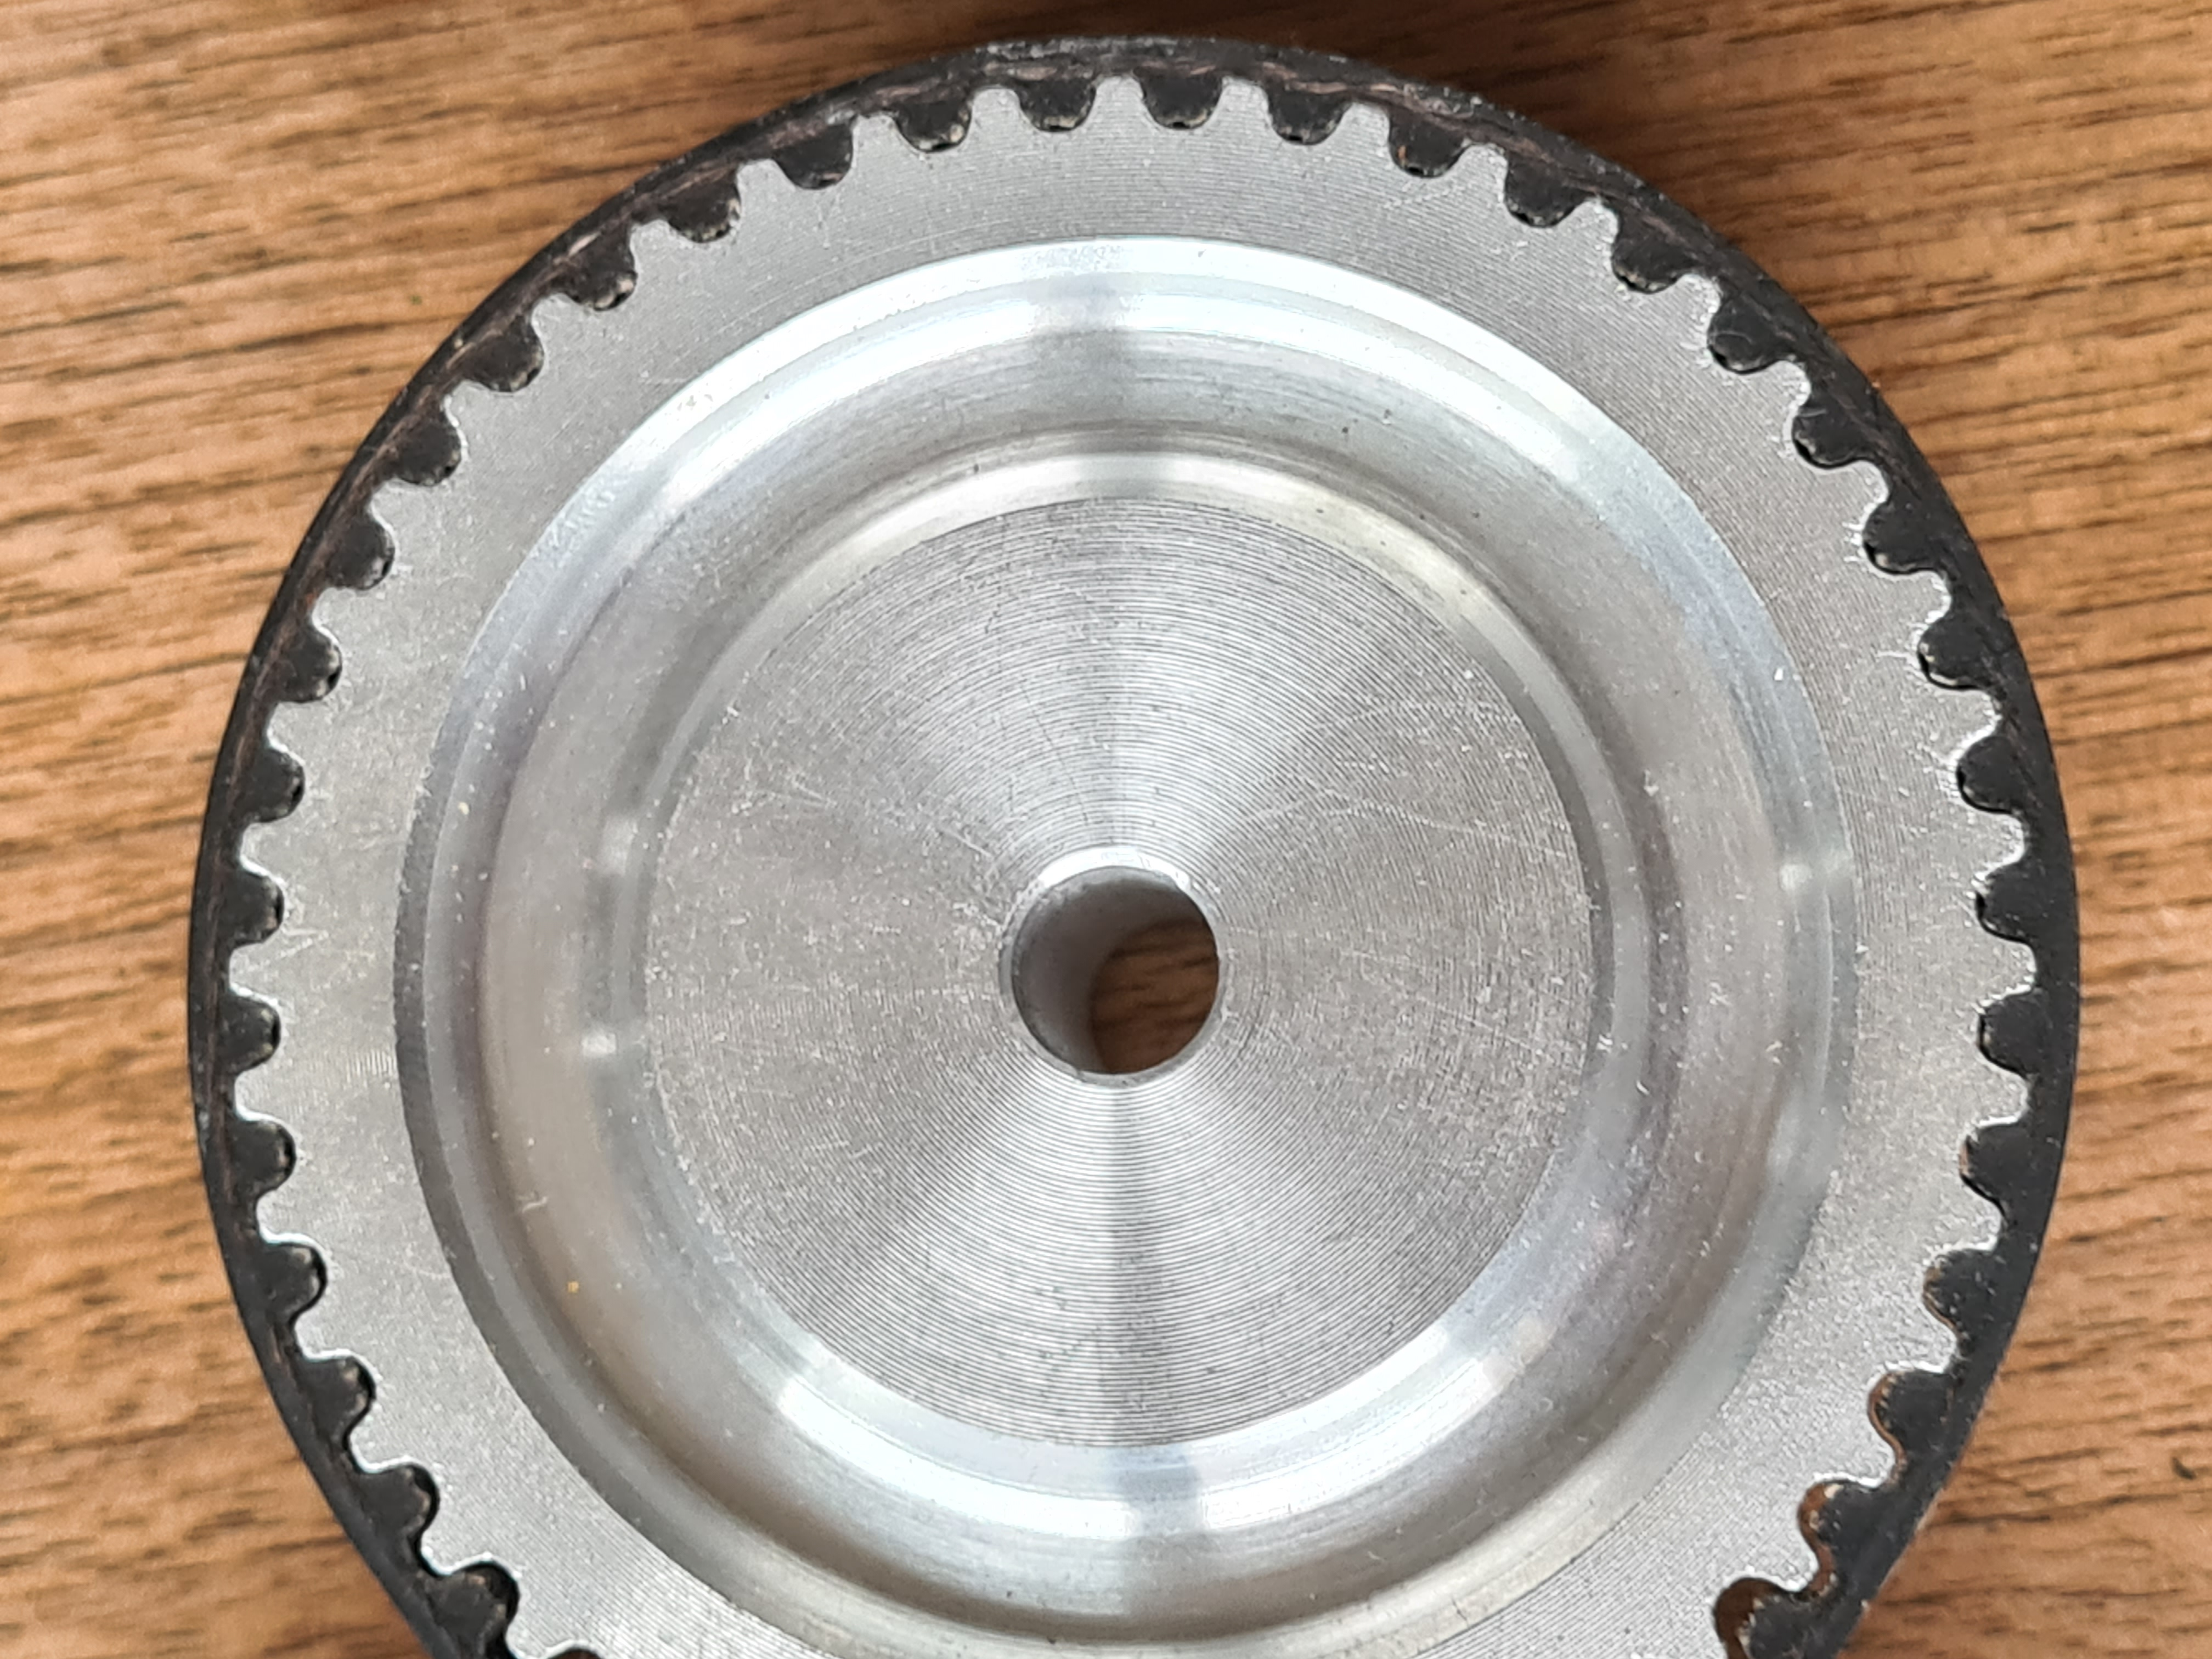
\includegraphics[width=\textwidth]{Footage/Pictures/Machined-HTD_tooth_fit.jpg}
				\caption{CNC-gefrästes HTD-Profil auf Riemen.}%
				\label{subfig:machined HTD}
			\end{subfigure}
			\hfill
			\begin{subfigure}{.49\textwidth}
				\centering
				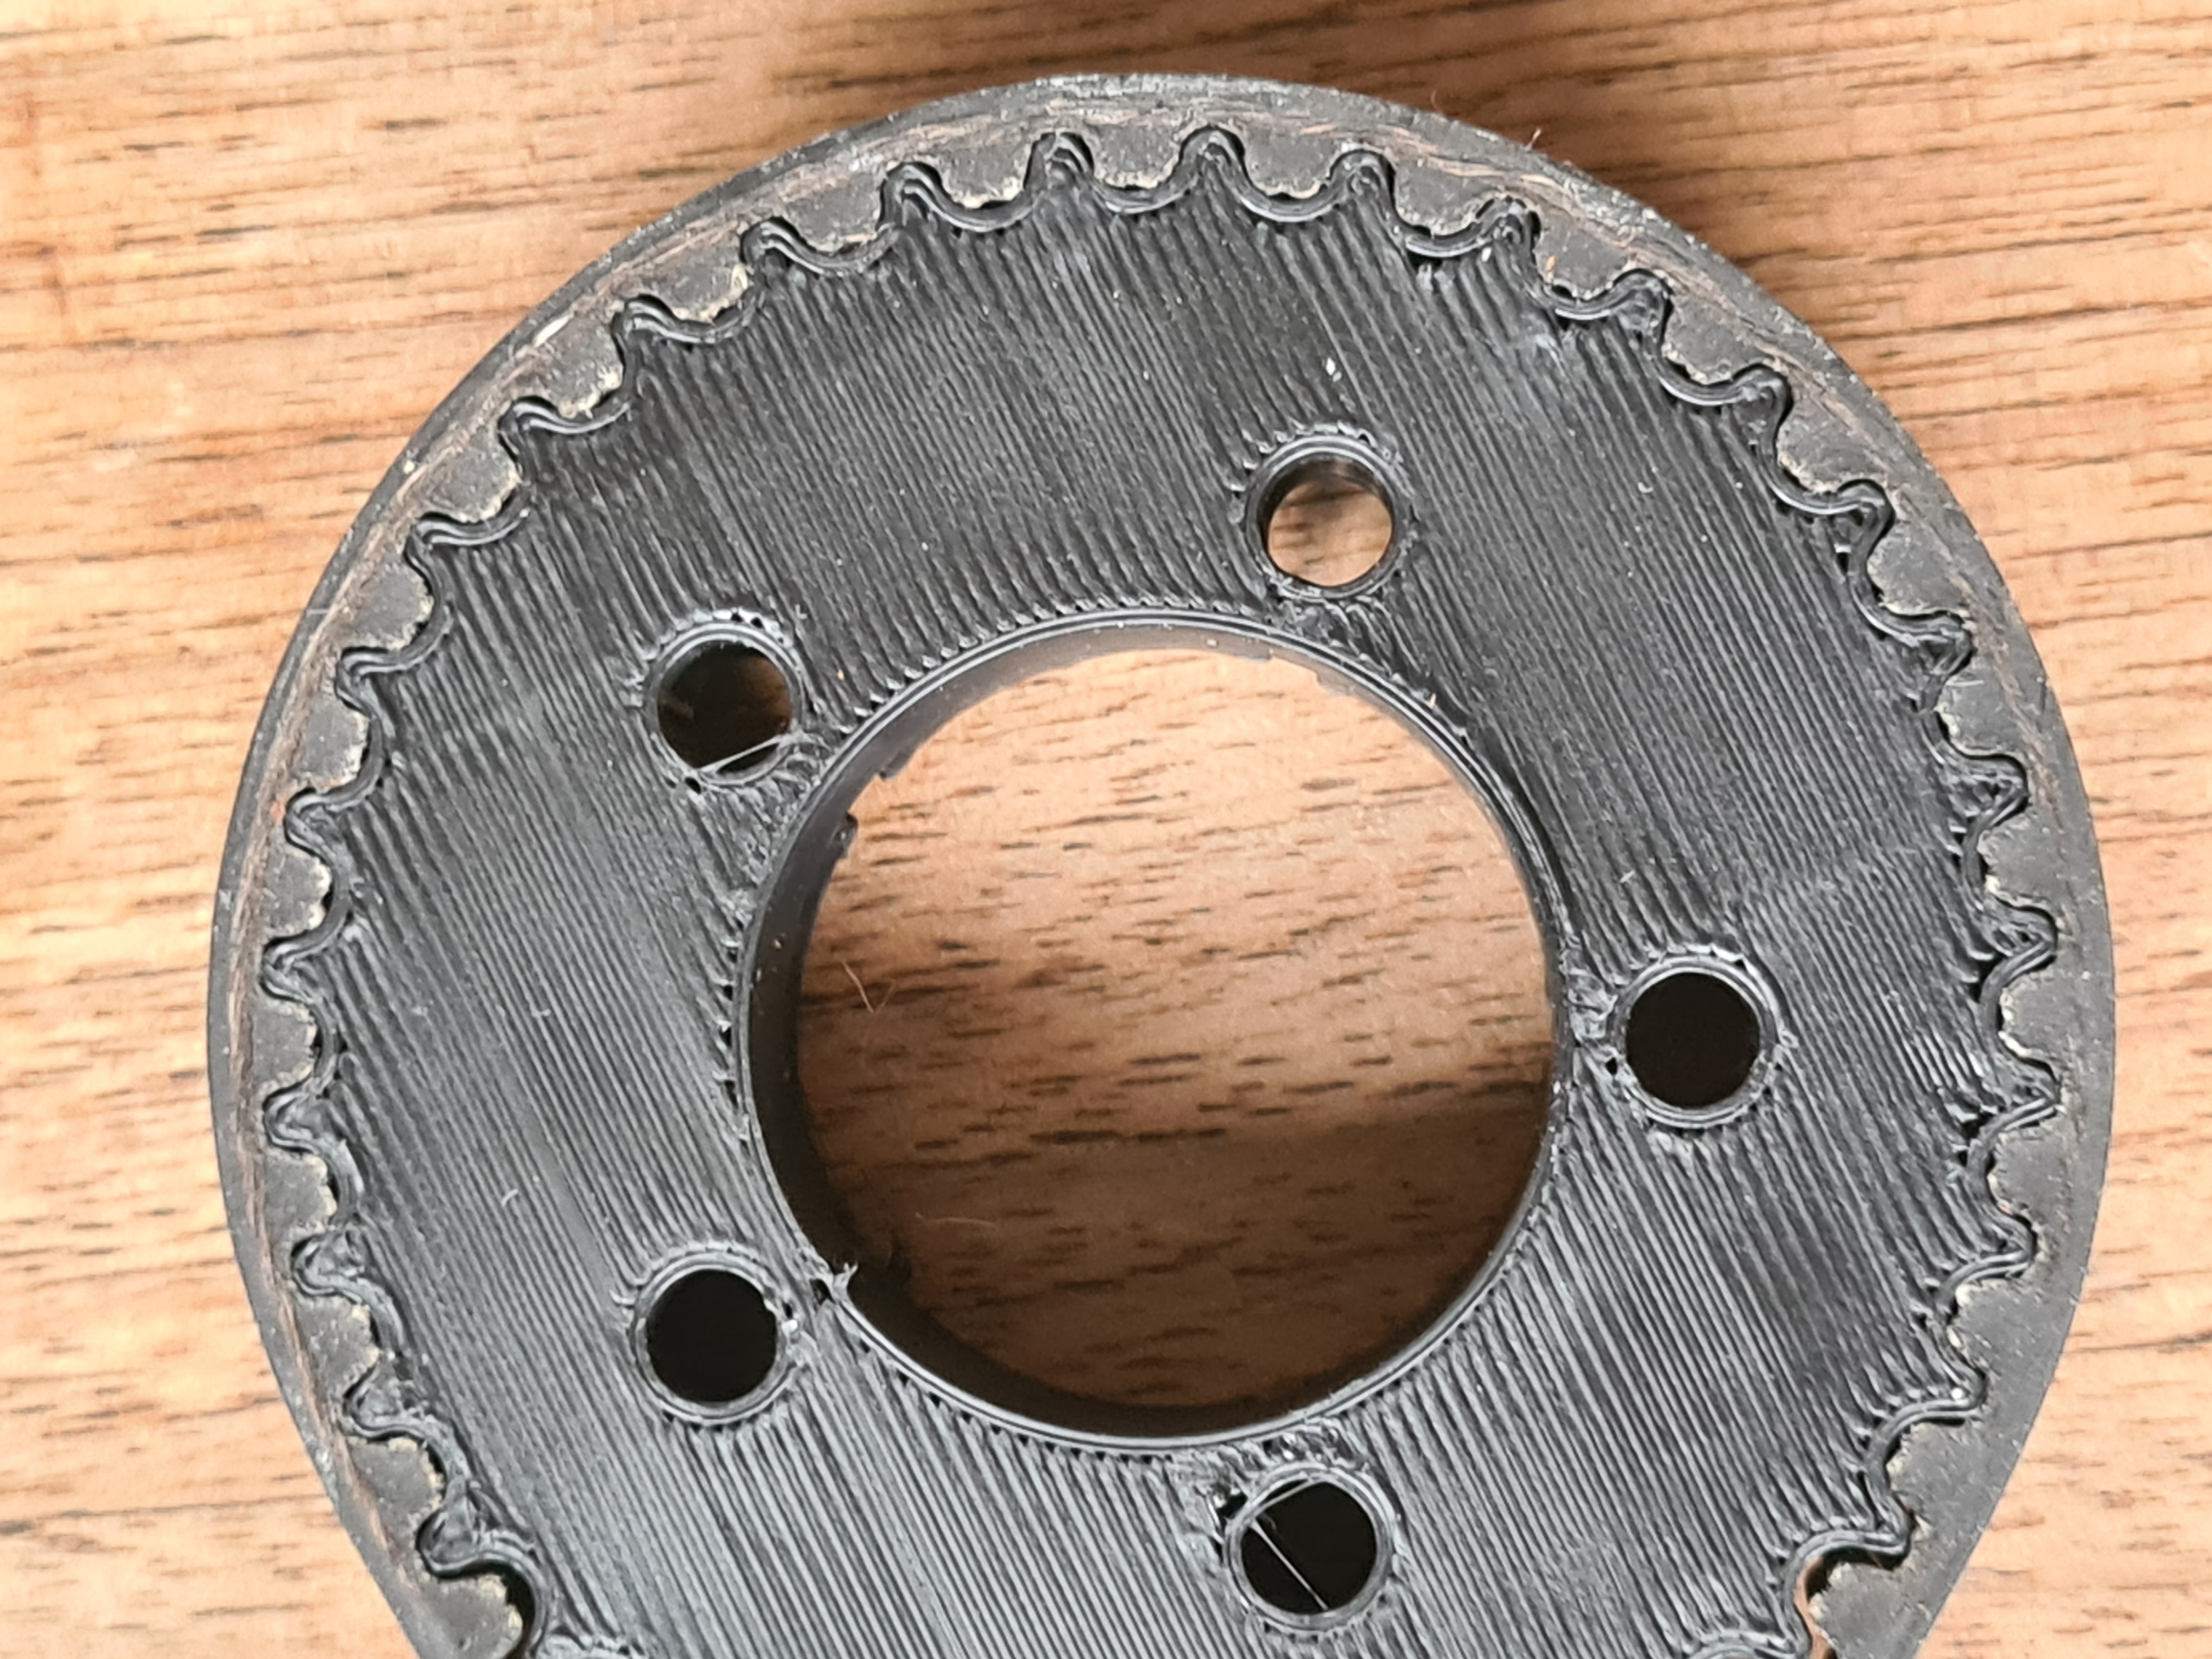
\includegraphics[width=\textwidth]{Footage/Pictures/Printed-HTD_tooth_fit.jpg}
				\caption{3D-gedrucktes HTD-Profil auf Riemen.}%
				\label{subfig:printed HTD}
			\end{subfigure}
			\caption{Vergleich der Passform einer gekauften Zahnscheibe (44T) aus Aluminium und des 3D-gedruckten Modells (36T) mit einem Riemen.}%
			\label{fig:HTD profiles comparison}
		\end{figure}\par\medskip
		%
		Da die Schrauben mit Muttern gekontert werden sollen und die der Zahnscheibe gegenüberliegende Seite der Rollen ebenfalls ein konkaves Profil aufweist, wurde ein komplementäres Gegenstück -- zu sehen in \cref{fig:orangatang kegel flat face} -- im oben beschriebenen Prozess modelliert.
		\begin{figure}[h]
			\centering
			\includesvg[width=.5\textwidth, inkscapelatex=false]{Footage/AwesomeBoard Transmission CAD/Drawings/Orangatang Kegel Flat Face}
			\caption[Zeichnung des Gegenstücks der Zahnscheibe]{Zeichnung des Gegenstücks der Zahnscheibe um eine ebene Fläche für die Muttern zur Verfügung zu stellen.}%
			\label{fig:orangatang kegel flat face}
		\end{figure}
		Wie auch die Zahnscheibe enthält die Konterscheibe fünf Bohrungen und fünf Führungsstifte und soll möglichst exakt dem inneren Profil der Rollen anliegen.
		
		Aus Kostengründen und einfachem Zugang zu den Betriebsmitteln wurde entschieden, die funktionalen Versionen der getriebeseitigen Zahn- und Konterscheibe ebenfalls im 3D-Druck-Verfahren aus ABS selbst herzustellen.
		Es ist zwar zu erwarten, dass die Zahnscheiben gegenüber aus Aluminium gefrästen Komponenten bezüglich Verschleiß und Festigkeit deutlich unterliegen, durch das gewählte Fertigungsverfahren lassen sich allerdings schnell, unkompliziert und günstig Ersatzteile herstellen.
		Darüber hinaus ist an dieser Stelle nicht mit einem plötzlichen Totalversagen der Materialintegrität zu rechnen.\par\medskip
		%
		Zur Auswahl des Riemens ist schließlich neben der Breite die Zahnung zu beachten.
		Ein vergrößerter Mittelpunktabstand beider Zahnscheiben erhöht grundsätzlich die Anzahl greifender Zähne, allerdings fällt dieser Effekt mit zunehmendem Abstand schnell ab.
		Es wurde ein Abstand so gewählt, dass zu jeder Zeit ein Zahn mehr als gefordert greift.
		Mit Zahnungen von 36T für die Antriebsseite, 15T getriebeseitig und dieser Vorgabe wurde eine Riemenzahnung von 55T gewählt.
		Die Riemenbreite wurde arbiträr auf \qty{12}{\milli\metre} und damit das breiteste käuflich erhältliche Maß festgelegt, dass konstruktiv umsetzbar ist.
		\Cref{fig:timing belt length} zeigt schematisch das System beider Zahnscheiben und Riemen.
		\begin{figure}[h]
			\centering
			\includesvg[width=.8\textwidth, inkscapelatex=false]{Footage/AwesomeBoard Transmission CAD/Drawings/Timing Belt assembly}
			\caption[Mittelpunktabstand zwischen antriebs- und getriebeseitigen Zahnscheiben]{Mittelpunktabstand zwischen antriebs- und getriebeseitigen Zahnscheiben bei einem Zahnriemen mit 55 Zähnen.}%
			\label{fig:timing belt length}
		\end{figure}
	\section{Motorbefestigung}\label{sec:motorbefestigung}
		Die Verbindung zwischen Motor und Hanger wurde in zwei Teilen hergestellt: eine Zange, die formschlüssig Verdrehen um die Hangerachse und durch Verspannen reibschlüssig Verschieben entlang der Hangerachse verhindert und ein Arm, der die Verbindung zwischen Zange und Motor herstellt.
		Kostenfreie Verfügbarkeit des Materials lässt die Werkstoffauswahl beider Komponenten auf Walzbleche der Aluminiumlegierung AlMgSi0,5 (EN AW 6060) fallen.
		Die Fertigung findet im CNC-Fräsverfahren statt.

		\begin{figure}[h]
			\centering
			\includesvg[width=.6\textwidth, inkscapelatex=false]{Footage/AwesomeBoard Transmission CAD/Drawings/Mount - Hanger Clamp}
			\caption[Zange zur Montage der Motorhalterung am Hanger]{Zange zur Montage der Motorhalterung am Hanger.}%
			\label{fig:hanger clamp drawing}
		\end{figure}
		\Cref{fig:hanger clamp drawing} zeigt eine Zeichnung der Zange mit allen relevanten Dimensionen.
		Erkennbar ist mittig eine Aussparung in Form des Profils des \textsc{Caliber II} Hangers mit Nut, um durch eine M5 Schraube an den beiden flachen Flanken des Hanger angespannt werden zu können.
		Um hier die Kontaktfläche zu maximieren wurde als Halbzeug ein Blech größtmöglicher, zur Verfügung stehender Materialstärke gewählt.
		Kreisförmig um die Rollachse des Hanger befinden sich sechs M4-Durchgangsbohrungen, um flach anliegend den Motorarm anbringen zu können.
		Drei Aussparungen entlang des äußeren Bogens sollen später Platz bieten, um Querverbindungen zwischen Armpaaren anbringen zu können.
		Sollte die Einspannung des Hangers in der Zange ein Driften entlang der bzw. Kippen gegen die Hangerachse nicht zuverlässig verhindern können, so sollen später an den drei Aussparungen entlang des äußeren Bogens Querverbindungen zwischen zwei gegenüberliegenden Zangen möglich sein.
		% Diese wiederum erfüllen einerseits den Zweck einer mechanischen Kopplung und damit einer Lastverteilung zwischen den Scheibe-Arm-Gruppen, andererseits wirken sie als Käfig zum Schutze der Motoren vor groben Schäden während der Fahrt wie etwa durch umherfliegendes Geröll oder Kontakt mit Bodenunebenheiten.

		\begin{figure}[h]
			\centering
			\includesvg[width=.7\textwidth, inkscapelatex=false]{Footage/AwesomeBoard Transmission CAD/Drawings/Mount - Motor Piece}
			\caption[Verbindungsarm zwischen Motor und Hangerzange]{Verbindungsarm zwischen Motor und Hangerzange. Wichtigste Merkmale: links radial um die Rollachse angeordnete Langlöcher zur Feinjustage des Montagewinkels. Rechts entlang der Längsachse des Armes ausgerichtete Langlöcher zur Justage der Riemenspannung.}%
			\label{fig:motor piece drawing}
		\end{figure}
		\newpage
		Ebenfalls aus AlMgSi0,5 und mit einer Materialstärke von \qty{4}{\milli\metre} stellt der Arm als komplementäre Komponente, flach an die Zange angeschraubt, eine steife Verbindung zwischen Hanger und Motor her.
		In \cref{fig:motor piece drawing} links befinden sich radial um die Rollachse angeordnet sechs Langlöcher zur Montage an der Zange.
		Da der gesamte Aufbau sich unterhalb des Decks befinden wird, ist es wichtig bezüglich der Motoren ein Optimum zwischen Bodenabstand und Distanz zum Deck zu finden.
		Um auch nach Zusammenbau die Abstände nachjustieren zu können, kann der Anstellwinkel des Armes innerhalb eines Winkels von \qty{22,5}{\degree} so auf einfache Weise angepasst werden.
		Rechts befinden sich vier weitere Langlöcher von \qty{6}{\milli\metre} Länge zur Befestigung des Motors.
		Hier dienen die Langlöcher der Möglichkeit nach Zusammenbau durch Variation des Abstandes von Roll- zu Motorachse die Riemenspannung nachjustieren zu können.
		Nach \cref{fig:timing belt length} ist mit der in \cref{sec:transmission} beschriebenen Konfiguration ein theoretischer Mittelpunktabstand von \(\approx \qty{74,34}{\milli\metre}\) zu erwarten.
		Der Mittelpunktabstand der Hangerachse und des Kreismittelpunktes der Langlöcher zur Motorbefestigung wurde mit \qty{73,5}{\milli\metre} so gewählt, dass bei einer Länge der Langlöcher von \qty{6}{\milli\metre} sowohl Ein- und Ausbau des Riemens, als auch adäquate Riemenspannung sichergestellt ist.

		Vier Bohrungen durch die äußeren Erhebungen um die Motorachse herum sollen es später ermöglichen bei Bedarf einen Riemenschutz anbringen zu können.
		Die Erhebungen selbst sollen den Zweck eines Puffermaterial im Falle eines Bodenkontaktes erfüllen.